
\section*{Interpolation}
\subsection*{Polinomial Interpolation}

\begin{algorithm}[H]
\SetAlgoLined
\DontPrintSemicolon
\KwIn{$x$: list of x coordinates, $y$: list of y coordinates, $u$: list of points where the interpolation is computed}
\KwOut{$v$: list of values of the interpolation at the points $u$}
$n \gets$ length of $x$;\\
$v \gets$ zeros vector with length of $u$;\\
\For{$i \gets 0$ \KwTo $n-1$}{
$w \gets$ ones vector with length of $u$;\\
\For{$j \gets 0$ \KwTo $n-1$}{
\If{$j \neq i$}{
$w \gets w * (u - x_j) / (x_i - x_j)$;
}
}
$v \gets v + w * y_i$
}
\Return $v$
\caption{Polinomial Interpolation}
\end{algorithm}
\subsubsection*{BNumMet Examples}
\paragraph{Example 1}{
\begin{lstlisting}[language=Python]
from BNumMet.Interpolation import polinomial
x = list(np.arange(1, 7, 1))
y = [16, 18, 21, 17, 15, 12]
u = np.arange(0.8, 6.2, 0.05)
v = polinomial(x, y, u)
# Plotting using Matplotlib
plt.plot(u, v, "b-", label="Interpolated")
plt.plot(x, y, "ro", label="Original Points")
plt.legend()
plt.show()
\end{lstlisting}
\begin{figure}[H]
    \centering
    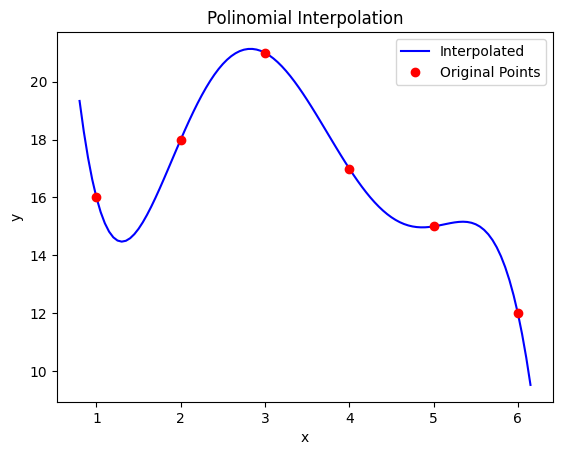
\includegraphics{Include/Images/Thesis/Documentation/Interpolation/Polinomial Example 1.png}
    \caption{Polinomial Linear Example 1}
    \label{fig:Polinomial Linear Example 1}
\end{figure}
}
\subsection*{Piecewise Linear Interpolation}

\begin{algorithm}[H]
\SetAlgoLined
\DontPrintSemicolon
\KwIn{$x$: list of x coordinates, $y$: list of y coordinates, $u$: list of points where the interpolation is computed, $sorted$: if the points are sorted or not (default: False)}
\KwOut{$v$: list of values of the interpolation at the points $u$}
\If{not $sorted$}{
$x \gets$ numpy array of $x$;\\
$y \gets$ numpy array of $y$;\\
$ind \gets$ indices of sorted $x$;\\
$x \gets x[ind]$;\\
$y \gets y[ind]$;\\
}
$\Delta \gets \text{diff}(y) / \text{diff}(x)$;\\
$n \gets$ length of $x$;\\
$k \gets$ zeros array with size of $u$, dtype=int;\\
\For{$j \gets 1$ \KwTo $n-2$}{
$k[x_j <= u] \gets j$
}
$s \gets u - x_k$\\
$v \gets y_k + s * \Delta_k$\\
\Return $v$
\caption{Piecewise Linear Interpolation}
\end{algorithm}
\subsubsection*{BNumMet Examples}
\paragraph{Example 1}{
\begin{lstlisting}[language=Python]
from BNumMet . Interpolation import piecewise_linear
x = list(np.arange(1, 7, 1))
y = [16, 18, 21, 17, 15, 12]
u = np.arange(0.8, 6.2, 0.05)
v = piecewise_linear(x, y, u)
# Plotting using Matplotlib
plt.plot(u, v, "b-", label="Interpolated")
plt.plot(x, y, "ro", label="Original Points")
plt.legend()
plt.show()
\end{lstlisting}
\begin{figure}[H]
    \centering
    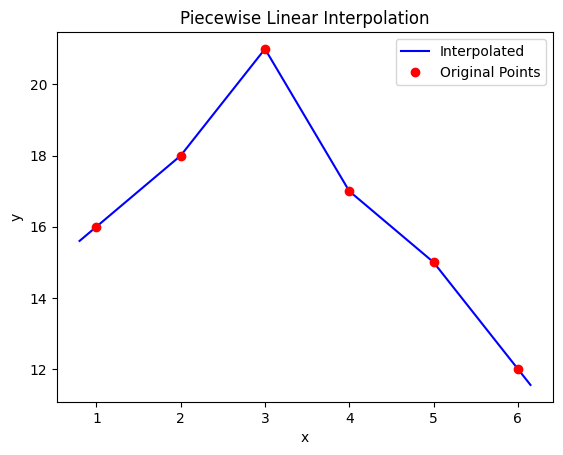
\includegraphics{Include/Images/Thesis/Documentation/Interpolation/PieceWise Linear Example 1.png}
    \caption{PieceWise Linear Example 1}
    \label{fig:PieceWise Linear Example 1}
\end{figure}
}

\subsection*{Piecewise Cubic Hermite Interpolation Polynomial (P.C.H.I.P.)}
The pchip function is a Python implementation of the Piecewise Cubic Hermite Interpolation Polynomial (P.C.H.I.P.) based on an old Fortran program by Fritsch and Carlson.

\begin{algorithm}[H]
\SetAlgoLined
\KwIn{List of x coordinates $x$, list of y coordinates $y$, list of points where the interpolation is computed $u$, and parameter to specify if the points are already sorted $sorted$}
\KwOut{List of values of the interpolation at the points $u$}
$n \leftarrow$ length of $x$;\\
$h \leftarrow x[1:n] - x[0:n-1]$;\\
$\delta \leftarrow (y[1:n] - y[0:n-1]) / h$;\\
$d \leftarrow \mathrm{pchip\_slopes}(h, \delta)$;\\
$v \leftarrow$ empty list;\\
\For{$i \leftarrow 1$ \KwTo $len(u)$}{
$j \leftarrow$ index such that $x_j \leq u_i \leq x_{j+1}$;\\
$b \leftarrow y[j] - d[j] \cdot h_j$;\\
$a \leftarrow (d[j+1] - d[j]) / (3 \cdot h_j)$;\\
$c \leftarrow \delta[j] - d[j] \cdot h_j - a \cdot h_j^2$;\\
$s \leftarrow a \cdot (u_i - x_j)^3 + d[j] \cdot (u_i - x_j)^2 + c \cdot (u_i - x_j) + b$;\\
append $s$ to $v$;\\
}
\Return $v$;

\medskip

\SetKwProg{Fn}{Function}{\string:}{}
\Fn{pchip\_slopes(h, delta)}{
$d \leftarrow$ array of zeros with length $n$;\\
$k \leftarrow$ indices of the points where the slopes are of the same sign, i.e., $\mathrm{sign}(\delta_{0:n-2}) \cdot \mathrm{sign}(\delta_{1:n-1}) > 0$;\\
$k \leftarrow k + 1$;\\
$w1 \leftarrow 2 \cdot h_k + h_{k-1}$;\\
$w2 \leftarrow h_k + 2 \cdot h_{k-1}$;\\
$d_k \leftarrow (w1 + w2) / (w1 / \delta_{k-1} + w2 / \delta_k)$;\\
$d_0 \leftarrow \mathrm{pchip\_end}(h_0, h_1, \delta_0, \delta_1)$;\\
append $\mathrm{pchip\_end}(h_{n-1}, h_{n-2}, \delta_{n-1}, \delta_{n-2})$ to $d$;\\
\Return $d$;
}

\medskip

\SetKwProg{Fn}{Function}{\string:}{}
\Fn{pchip\_end(h1, h2, delta1, delta2)}{
$d \leftarrow ((2 \cdot h1 + h2) \cdot \delta1 - h1 \cdot \delta2) / (h1 + h2)$;\\

\If{$\mathrm{sign}(\delta1) \neq \mathrm{sign}(\delta2)$ or $\left|d\right| > 3\cdot\left|\delta1\right|$ or $\left|d\right| > 3\cdot\left|\delta2\right|$}{
$d \leftarrow 0$
}
\KwRet{$d$}
}
\caption{Piecewise Cubic Hermite Interpolation}
\end{algorithm}

\subsubsection*{BNumMet Examples}
\paragraph{Example 1}{
\begin{lstlisting}[language=Python]
from BNumMet.Interpolation import pchip
x = list(np.arange(1, 7, 1))
y = [16, 18, 21, 17, 15, 12]
u = np.arange(0.8, 6.2, 0.05)
v = pchip(x, y, u)
# Plotting using Matplotlib
plt.plot(u, v, "b-", label="Interpolated")
plt.plot(x, y, "ro", label="Original Points")
plt.legend()
plt.show()
\end{lstlisting}

\begin{figure}[H]
    \centering
    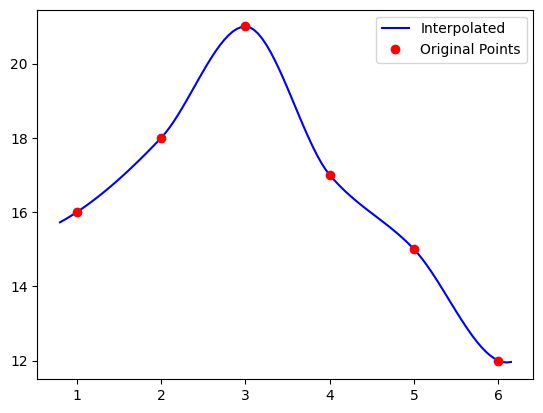
\includegraphics{Include/Images/Thesis/Documentation/Interpolation/PCHIP Example 1.png}
    \caption{PCHIP Example 1}
    \label{fig:PCHIP Example 1}
\end{figure}
}

\subsection*{Piecewise cubic Interpolatory Splines}
\begin{algorithm}[H]
\SetAlgoLined
\KwIn{List of x coordinates $x$, list of y coordinates $y$, list of points where the interpolation is computed $u$, and parameter to specify if the points are already sorted $sorted$}
\KwOut{List of values of the interpolation at the points $u$}
$n \leftarrow$ length of $x$;\\
$h \leftarrow x[1:n] - x[0:n-1]$;\\
$\delta \leftarrow (y[1:n] - y[0:n-1]) / h$;\\
$d \leftarrow \mathrm{splineslopes}(h, \delta)$;\\
$v \leftarrow$ empty list;\\
\For{$i \leftarrow 1$ \KwTo $len(u)$}{
$j \leftarrow$ index such that $x_j \leq u_i \leq x_{j+1}$;\\
$b \leftarrow y[j] - d[j] \cdot h_j$;\\
$a \leftarrow (d[j+1] - d[j]) / (3 \cdot h_j)$;\\
$c \leftarrow \delta[j] - d[j] \cdot h_j - a \cdot h_j^2$;\\
$s \leftarrow a \cdot (u_i - x_j)^3 + d[j] \cdot (u_i - x_j)^2 + c \cdot (u_i - x_j) + b$;\\
append $s$ to $v$;\\
}
\Return $v$;

\SetKwProg{Fn}{Function}{ is}{end}
\Fn{\texttt{splineslopes}$(h, \delta)$}{

$a \leftarrow \mathrm{zeros}(len(h))$; $b \leftarrow \mathrm{zeros}(len(h))$; $c \leftarrow \mathrm{zeros}(len(h))$; $r \leftarrow \mathrm{zeros}(len(h))$ ;

$a[:-1] \leftarrow h[1:]$ ;\\
$a[-1] \leftarrow h[-2] + h[-1]$ ;\\
$b[0] \leftarrow h[1]$ ;\\
$b[1:] \leftarrow 2 \cdot (h[1:] + h[:-1])$;\\
$\mathrm{append}(b, h[-2])$ ;\\
$c[0] \leftarrow h[0] + h[1]$;\\
$c[1:] \leftarrow h[:-1]$ ;\\
$r[0] \leftarrow ((h[0] + 2 \cdot c[0]) \cdot h[1] \cdot \delta[0] + h[0] ^ 2 \cdot \delta[1]) / c[0]$ ;\\
$r[1:] \leftarrow 3 \cdot (h[1:] \cdot \delta[:-1] + h[:-1] \cdot \delta[1:])$ ;\\
$\mathrm{append}(r, (h[-1] ^ 2 \cdot \delta[-2] + (2 \cdot a[-1] + h[-1]) \cdot h[-2] \cdot \delta[-1]) / a[-1])$; \\
$res \leftarrow \mathrm{lu\_solve}(\mathrm{diag}(a, -1) + \mathrm{diag}(b) + \mathrm{diag}(c, 1), r)$ ;\\
\KwRet $res.\mathrm{astype}(float)$ ;
}
\caption{Piecewise cubic Interpolatory Splines}
\end{algorithm}

\subsubsection*{BNumMet Examples}
\paragraph{Example 1}{
\begin{lstlisting}[language=Python]
from BNumMet.Interpolation import splines
x = list(np.arange(1, 7, 1))
y = [16, 18, 21, 17, 15, 12]
u = np.arange(0.8, 6.2, 0.05)
v = splines(x, y, u)
# Plotting using Matplotlib
plt.plot(u, v, "b-", label="Interpolated")
plt.plot(x, y, "ro", label="Original Points")
plt.legend()
plt.show()
\end{lstlisting}
\begin{figure}[H]
    \centering
    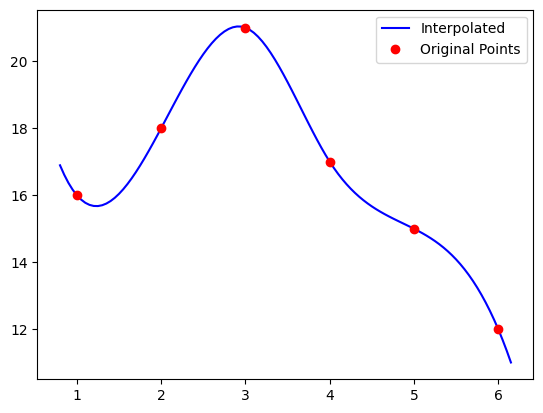
\includegraphics{Include/Images/Thesis/Documentation/Interpolation/Splines Example 1.png}
    \caption{Splines Example 1}
    \label{fig:Splines Example 1}
\end{figure}

}